\chapter{Analiză și fundamentare teoretică}
\label{ch:analysis}
\pagestyle{fancy}

În capitolul precedent au fost prezentate proiectele și tehnologiile pe care se
sprijină lucrarea de față. Acest capitol coboară cu un nivel mai jos și explică,
din punct de vedere teoretic, modul în care funcționează fiecare verigă a
sistemului de control. Sunt analizate, pe rând, structura logică a întregului
lanț de prelucrare a semnalului, principiul mecanic prin care comenzile electrice
se transformă în mișcarea degetelor, protocolul prin care calculatorul comunică
cu placa, modelul matematic al filtrului Kalman, aritmetica folosită pentru a-l
implementa pe o platformă fără unitate în virgulă mobilă, generarea semnalelor de
comandă pentru servomotoare, constrângerile temporale impuse de funcționarea în
timp real și, în final, raționamentul care a stat la baza alegerii componentelor
electronice. Accentul cade aici pe principii și pe relațiile matematice care le
descriu, urmând ca modul concret în care acestea au fost transpuse în hardware să
fie tratat în capitolul de proiectare și implementare.

\section{Structura logică a sistemului}
\label{sec:analiza-structura}

Sistemul poate fi privit ca un lanț prin care o mișcare a mâinii umane este
transformată, pas cu pas, într-o mișcare echivalentă a mâinii robotice. La un
capăt al lanțului se află un calculator care urmărește mâna operatorului cu
ajutorul unei camere web, iar la celălalt capăt se găsesc cele opt servomotoare
care acționează degetele și articulațiile brațului. Între cele două extreme se
află placa FPGA, care primește datele, le filtrează și generează semnalele
de comandă. Această împărțire pe niveluri este reprezentată în
Figura~\ref{fig:schema-bloc}.

\begin{figure}[H]
	\centering
	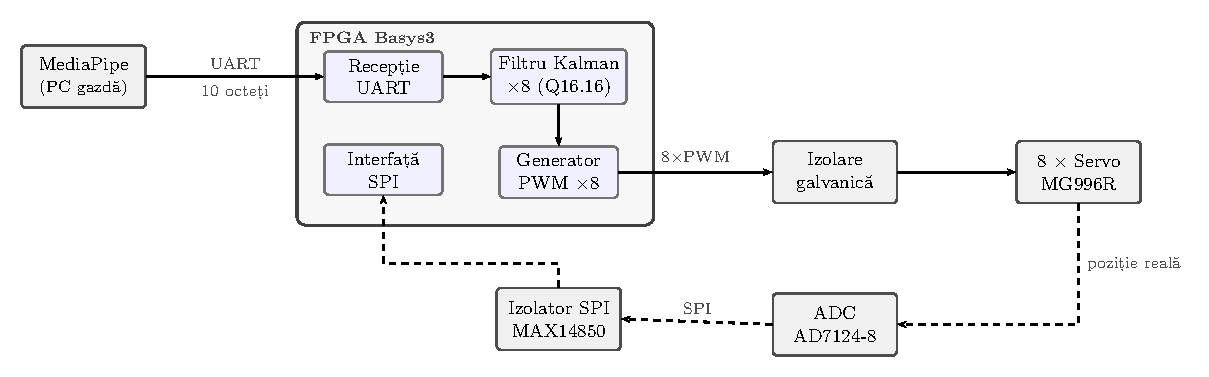
\includegraphics[width=0.95\textwidth]{figs/schema_bloc.pdf}
	\caption{Structura logică a sistemului de control, cu fluxul principal de
	comandă (linie continuă) și bucla de monitorizare prin convertorul
	analog-digital (linie întreruptă).}
	\label{fig:schema-bloc}
\end{figure}

Partea de viziune artificială, realizată de colegul meu, rulează pe calculatorul
gazdă și se ocupă cu detecția poziției articulațiilor mâinii din fluxul video.
Rezultatul acestei prelucrări este un set de opt unghiuri, câte unul pentru
fiecare grad de libertate al mâinii robotice, exprimate ca valori întregi între 0
și 180 de grade. Aceste unghiuri reprezintă, practic, comanda brută de poziție pe
care sistemul trebuie să o reproducă. Ele sunt împachetate într-un cadru și
trimise prin interfața serială UART către placa FPGA, despre care voi vorbi pe
larg în secțiunea dedicată protocolului de comunicație.

Odată ajunse pe placă, datele intră în partea centrală a sistemului, cea care
constituie de fapt contribuția mea. Aici, un modul de recepție extrage unghiurile
din cadrul primit și verifică integritatea acestora, după care valorile sunt
preluate de filtrul Kalman. Filtrul tratează fiecare canal de servo în mod
independent și are rolul de a netezi comenzile, eliminând variațiile bruște și
zgomotul provenit din procesul de detecție vizuală. Pornind de la unghiurile
filtrate, un generator dedicat produce cele opt semnale de tip PWM care comandă
poziția servomotoarelor. Toate aceste module funcționează în paralel în interiorul
circuitului, sincronizate de același ceas de sistem.

Semnalele de comandă nu ajung însă direct la servomotoare. Ele traversează mai
întâi o barieră de izolare galvanică, al cărei rol este de a separa complet
domeniul digital, sensibil, al plăcii FPGA de domeniul de putere, mult mai
zgomotos, în care lucrează motoarele. Abia după această izolare semnalele ajung la
servomotoare și produc mișcarea efectivă a degetelor.

În paralel cu fluxul principal de comandă există și o cale de întoarcere,
reprezentată în figură prin linia întreruptă. Un convertor analog-digital citește
poziția reală a servomotoarelor și transmite aceste valori înapoi către placă,
tot printr-o interfață izolată. Este important de subliniat că această cale are
rol de monitorizare, nu de control în buclă închisă. Ea permite observarea
poziției efective a articulațiilor, fără a interveni direct în generarea
comenzilor, motiv pentru care a fost reprezentată distinct față de lanțul
principal.

Întregul sistem funcționează ritmat de un ciclu fix de 20 de milisecunde, valoare
impusă de modul în care servomotoarele standard interpretează semnalul de comandă.
La fiecare astfel de ciclu se preia cel mai recent set de unghiuri disponibil, se
aplică filtrarea și se actualizează semnalele de ieșire. Acest ritm constituie
referința temporală a întregului sistem și va reveni de mai multe ori pe parcursul
capitolului, fiind elementul în jurul căruia se construiește analiza temporală din
secțiunea dedicată.

\section{Modelul de acționare a mâinii}
\label{sec:analiza-actionare}

Înainte de a discuta despre partea electronică, este util să înțelegem cum se
transformă o comandă unghiulară a unui servomotor în îndoirea efectivă a unui
deget. Mâna robotică folosită în această lucrare reproduce, într-o formă
simplificată, mecanismul natural al mâinii umane, în care degetele sunt acționate
prin tendoane. Modelul de funcționare este ilustrat în
Figura~\ref{fig:mecanism}.

\begin{figure}[H]
	\centering
	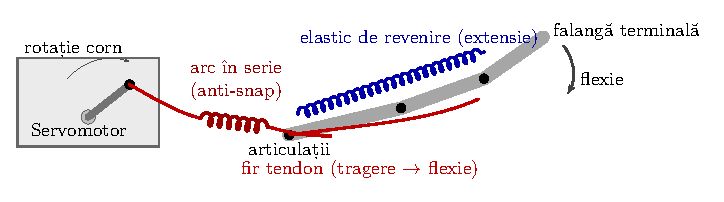
\includegraphics[width=0.85\textwidth]{figs/mecanism_actionare.pdf}
	\caption{Principiul de acționare a unui deget prin tendon. Servomotorul trage
	de firul care îndoaie degetul, iar elasticul de pe partea dorsală readuce
	degetul în poziția inițială.}
	\label{fig:mecanism}
\end{figure}

Fiecare deget este acționat de un singur servomotor, care joacă rolul mușchiului.
Cornul rotativ al servomotorului trage de un fir ce traversează degetul pe partea
palmară, exact așa cum tendoanele flexoare trag de oasele degetului uman. Atunci
când servomotorul se rotește, firul este tras, iar degetul se îndoaie. Revenirea
în poziția deschisă nu se face printr-un al doilea fir, ci pasiv, cu ajutorul unui
element elastic montat pe partea dorsală a degetului, care preia rolul tendonului
extensor. În felul acesta, un singur motor este suficient pentru a controla
închiderea și deschiderea unui deget, ceea ce simplifică mult mecanismul.

Firul care joacă rolul tendonului nu este unul oarecare. Pentru această funcție am
ales un fir de pescuit din categoria celor cu rezistență ridicată și memorie
redusă, cu un diametru de 0,27~mm și o rezistență la rupere de 14~kg, prezentat în
Figura~\ref{fig:fir}. Diametrul mic îi permite să alunece ușor prin canalele de
ghidare din interiorul degetelor, iar rezistența ridicată asigură că firul suportă
fără probleme forțele dezvoltate de servomotor, chiar și atunci când degetul
întâmpină rezistență. Memoria redusă a firului este de asemenea importantă,
deoarece un fir care și-ar păstra forma de pe mosor ar introduce o tensiune
suplimentară, nedorită, în mecanism.

\begin{figure}[H]
	\centering
	
\includegraphics[width=0.45\textwidth]{figs/fir_pescuit.jpg}
	\caption{Firul de pescuit folosit pe post de tendon, cu diametrul de 0,27~mm
	și rezistența la rupere de 14~kg.}
	\label{fig:fir}
\end{figure}

Un detaliu important al mecanismului îl reprezintă modul în care firul este legat
de servomotor. Între corn și deget, pe traseul firului, este montat în serie un
arc elicoidal de extensie, asemănător celui prezentat în
Figura~\ref{fig:arc}. La prima vedere ar putea părea un element în plus, însă
rolul său este esențial. Servomotorul este un actuator rigid, care se deplasează
exact în poziția comandată, fără a ceda. Dacă firul ar fi legat direct, orice
comandă care ar cere o tragere mai mare decât permite degetul, sau orice blocare
mecanică a acestuia, ar solicita brusc firul și articulațiile, putând duce la
ruperea firului sau la deteriorarea pieselor printate. Arcul montat în serie preia
aceste vârfuri de tensiune, întinzându-se atunci când forța depășește o anumită
valoare și protejând astfel întregul ansamblu. El se comportă ca un element de
siguranță elastic, care absoarbe șocurile și evită ruperea bruscă a firului.

\begin{figure}[H]
	\centering
	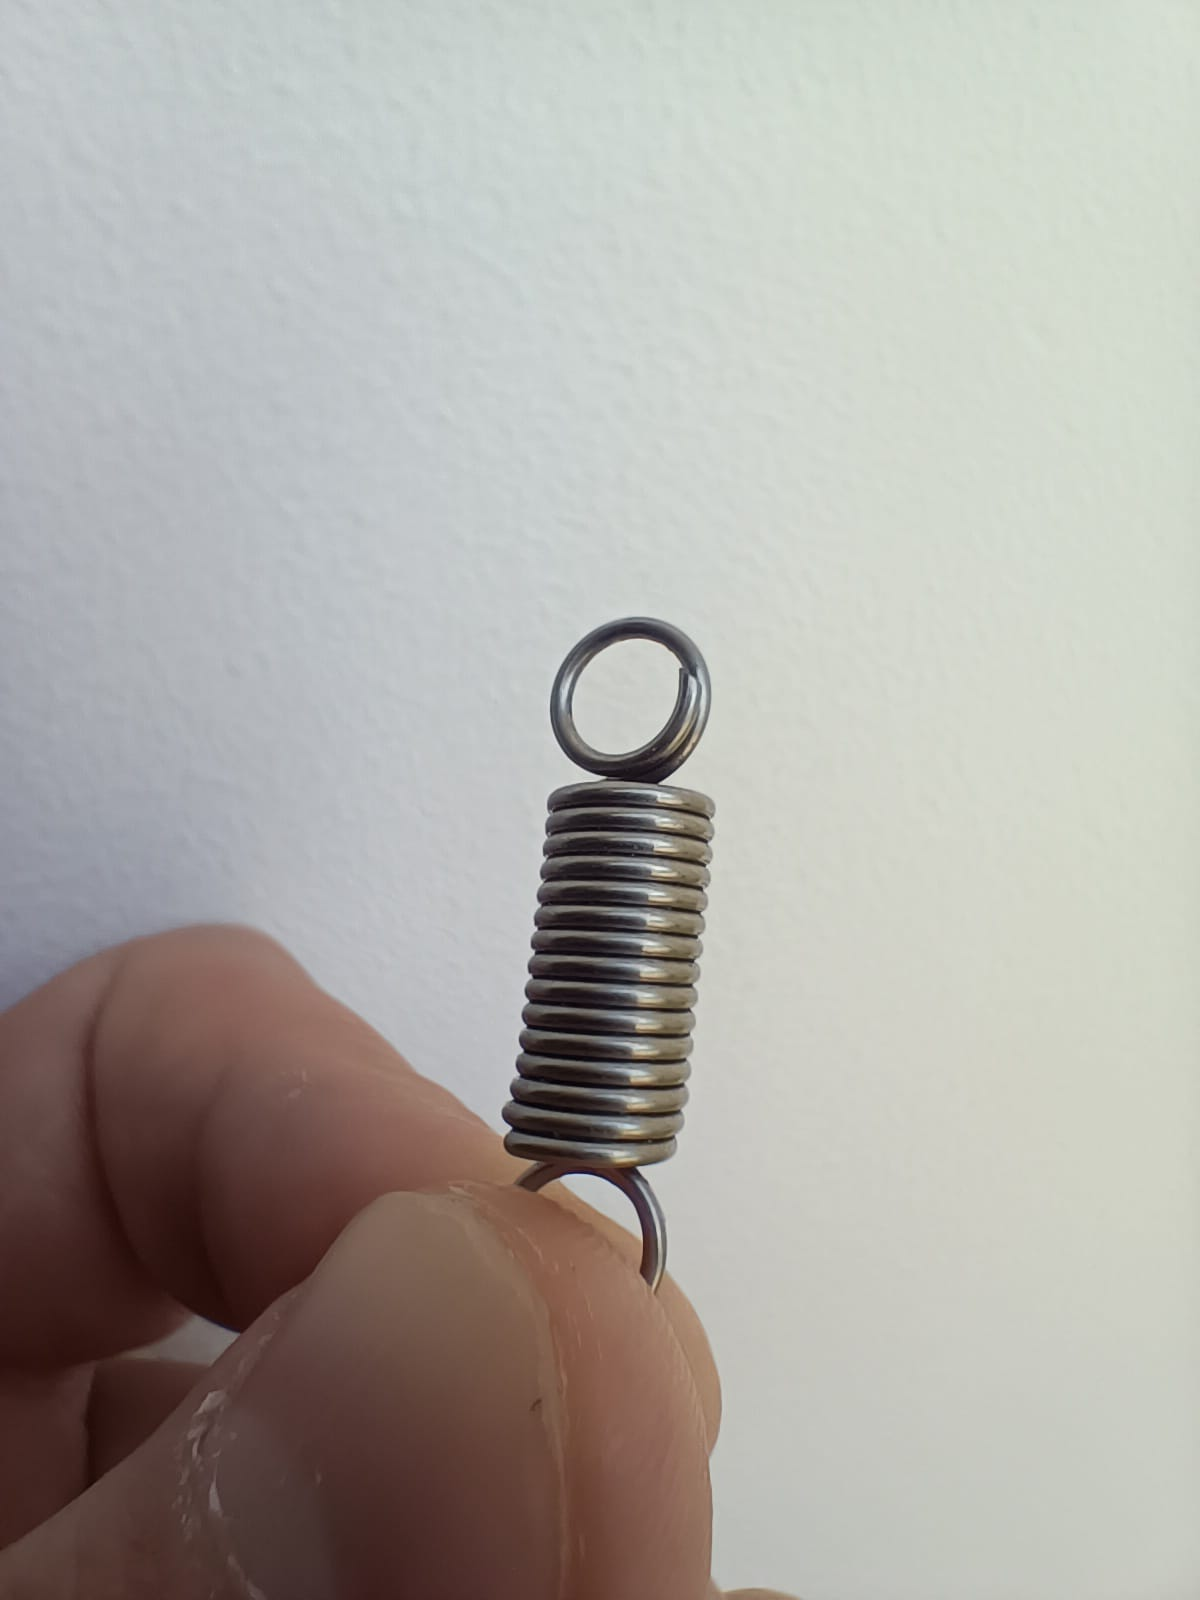
\includegraphics[width=0.4\textwidth]{figs/arc_tensiune.jpg}
	\caption{Arcul de extensie montat în serie pe firul de acționare, cu rolul de
	a prelua vârfurile de tensiune și de a proteja mecanismul.}
	\label{fig:arc}
\end{figure}

Pe lângă acționarea degetelor, același principiu bazat pe fire și scripeți este
folosit și pentru rotația încheieturii. Un servomotor dedicat rotește un sistem de
scripeți care permite întoarcerea palmei, reproducând mișcarea de rotație a
mâinii umane. Modul concret în care toate aceste elemente au fost dimensionate și
asamblate, împreună cu detaliile mecanice ale ansamblului, este tratat în
capitolul de proiectare. Aici interesează doar principiul de funcționare, fiindcă
el explică legătura dintre unghiul calculat de filtrul Kalman și mișcarea fizică
pe care sistemul trebuie să o producă. Modelul cinematic detaliat al mecanismului
de acționare prin tendoane a fost studiat pe larg de Hussein în lucrarea sa
\cite{hussein2014}, de la care a fost preluată și o parte din structura mecanică a
brațului.

\section{Protocolul de comunicație UART}
\label{sec:analiza-uart}

Legătura dintre calculatorul gazdă și placa FPGA se realizează prin interfața
serială UART, o alegere motivată de simplitatea și fiabilitatea acestui protocol.
UART nu necesită un semnal de ceas separat între cele două capete, ci se bazează
pe o rată de transfer convenită dinainte, ceea ce reduce numărul de fire necesare
la doar două, unul pentru fiecare sens de comunicație. În cazul de față se
folosește o configurație clasică, cu o rată de 115200 de biți pe secundă, opt biți
de date, fără bit de paritate și un singur bit de stop. Această configurație este
îndeobște notată prescurtat 8N1 și reprezintă un compromis bun între viteză și
robustețe pentru distanțele scurte din interiorul montajului.

Datele nu sunt trimise octet cu octet la întâmplare, ci grupate într-un cadru cu o
structură fixă. Fiecare cadru transportă unghiurile pentru toate cele opt
servomotoare, împreună cu informația necesară pentru a delimita începutul cadrului
și pentru a verifica integritatea datelor. Structura aleasă este reprezentată în
Figura~\ref{fig:cadru-uart} și cuprinde zece octeți.

\begin{figure}[H]
	\centering
	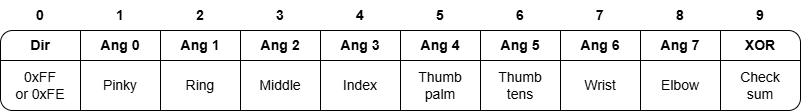
\includegraphics[width=0.95\textwidth]{figs/cadru_uart.png}
	\caption{Structura cadrului UART de zece octeți. Primul octet indică direcția,
	urmează cele opt unghiuri articulare, iar ultimul octet conține suma de
	control.}
	\label{fig:cadru-uart}
\end{figure}

Primul octet al cadrului are rol de antet și de delimitator. El indică direcția
transferului, distingând între o comandă prin care calculatorul trimite unghiuri
noi către placă și o cerere prin care se solicită citirea valorilor curente.
Urmează opt octeți, câte unul pentru fiecare articulație, în ordinea degetelor de
la cel mic până la degetul mare, urmate de rotația încheieturii și de extensia
cotului. Fiecare astfel de octet codifică un unghi cuprins între 0 și 180 de
grade, valoare care încape exact pe un octet și nu necesită o reprezentare mai
complexă. Ultimul octet al cadrului este o sumă de control, calculată ca SAU
exclusiv al tuturor octeților anteriori, și servește la detectarea eventualelor
erori de transmisie.

Mecanismul sumei de control este simplu, dar eficient. La emisie, calculatorul
combină prin SAU exclusiv toți cei nouă octeți de date și plasează rezultatul în
ultimul octet. La recepție, placa repetă același calcul pe octeții primiți și
compară rezultatul cu valoarea primită. Dacă vreun bit a fost alterat pe parcursul
transmisiei, cele două valori nu mai coincid, iar cadrul este respins. Proprietatea
matematică pe care se sprijină această verificare este aceea că orice valoare
combinată prin SAU exclusiv cu ea însăși produce zero, astfel încât SAU exclusiv al
tuturor celor zece octeți ai unui cadru corect trebuie să fie întotdeauna nul.
Această metodă detectează toate erorile care afectează un singur bit și are
avantajul că se calculează extrem de ușor în hardware, cu o singură operație logică
pe ciclu de ceas.

Merită analizat și timpul necesar transmiterii unui cadru, pentru că el trebuie să
se încadreze confortabil în ciclul de control al sistemului. În formatul 8N1,
fiecare octet ocupă de fapt zece biți pe linia serială, fiindcă la cei opt biți de
date se adaugă bitul de start și bitul de stop. Un cadru complet de zece octeți
înseamnă astfel o sută de biți transmiși. La rata de 115200 de biți pe secundă,
timpul de transmisie al unui cadru întreg este de aproximativ 0,87~ms, adică sub
cinci procente din ciclul de 20~ms al sistemului. Rămâne deci un interval larg
între momentul sosirii unui cadru și momentul în care valorile trebuie folosite,
ceea ce simplifică mult sincronizarea dintre recepție și prelucrare, aspect tratat
în detaliu în secțiunea dedicată analizei temporale.

\section{Filtrul Kalman cu două stări}
\label{sec:analiza-kalman}

Filtrul Kalman reprezintă componenta centrală a prelucrării realizate pe placă.
Rolul său este de a transforma unghiurile brute, primite de la sistemul de viziune
și afectate de zgomot, într-o traiectorie netedă, care urmărește fidel mișcarea
reală a mâinii operatorului fără a reproduce variațiile bruște și artefactele
detecției vizuale. Principiul general al filtrului și ecuațiile sale în formă
matriceală au fost prezentate în capitolul de studiu bibliografic. În cele ce
urmează, filtrul este particularizat pentru cazul concret al acestui proiect, în
care fiecare servomotor este modelat printr-un sistem cu două stări.

\subsection{Alegerea modelului cu două stări}

Pentru fiecare canal de servo se urmărește estimarea a două mărimi, poziția
unghiulară și viteza unghiulară. Poziția este mărimea care interesează direct,
fiindcă ea determină comanda trimisă servomotorului, în timp ce viteza este o
mărime auxiliară, care permite filtrului să anticipeze evoluția mișcării între
două măsurători succesive. Vectorul de stare conține așadar aceste două
componente,

\begin{equation}
\label{eq:kalman-stare}
\mathbf{x} =
\begin{bmatrix} x_0 \\ x_1 \end{bmatrix} =
\begin{bmatrix} \text{poziție} \\ \text{viteză} \end{bmatrix} ,
\end{equation}

unde $x_0$ reprezintă unghiul curent, exprimat în grade, iar $x_1$ reprezintă
viteza de variație a acestuia, exprimată în grade pe secundă.

Alegerea unui model cu exact două stări nu este întâmplătoare. Un model cu o
singură stare, care ar reține doar poziția, nu ar putea anticipa în niciun fel
mișcarea și s-ar comporta ca o simplă mediere a măsurătorilor, întârziind răspunsul
la mișcările rapide ale mâinii. La cealaltă extremă, un model cu trei stări, care
ar adăuga și accelerația, ar urmări mai fidel mișcările complexe, dar ar fi mai
sensibil la zgomot și ar necesita un volum mai mare de calcule. Pentru o mână
robotică ce urmărește gesturi umane, modelul cu două stări oferă cel mai bun
echilibru, fiind suficient de expresiv pentru a anticipa mișcarea, dar destul de
simplu pentru a fi implementat eficient în hardware.

\subsection{Modelul de evoluție}

Trecerea de la un moment de timp la următorul se face pe baza unui model cinematic
simplu, în care se presupune că viteza rămâne aproximativ constantă pe durata unui
interval de eșantionare $\Delta t$. Poziția la momentul următor este atunci poziția
curentă, la care se adaugă distanța parcursă la viteza estimată, iar viteza rămâne
neschimbată,

\begin{align}
\label{eq:kalman-evolutie}
x_0(k+1) &= x_0(k) + \Delta t \cdot x_1(k) , \\
x_1(k+1) &= x_1(k) .
\end{align}

Aceste relații se scriu compact cu ajutorul matricei de tranziție $\mathbf{F}$,
sub forma $\mathbf{x}(k+1) = \mathbf{F}\,\mathbf{x}(k)$, unde

\begin{equation}
\label{eq:kalman-F}
\mathbf{F} =
\begin{bmatrix} 1 & \Delta t \\ 0 & 1 \end{bmatrix} .
\end{equation}

Intervalul de eșantionare $\Delta t$ coincide cu ciclul de control al sistemului,
adică 0,02 secunde, fiindcă filtrul este actualizat o singură dată la fiecare ciclu
de 20~ms. Presupunerea de viteză constantă este o aproximație, însă pe un interval
atât de scurt ea este pe deplin justificată, iar abaterile de la acest model sunt
tratate de filtru prin intermediul zgomotului de proces.

\subsection{Modelul de măsurare}

Mărimea pe care sistemul o măsoară efectiv este doar poziția unghiulară, nu și
viteza. Relația dintre starea sistemului și măsurătoare se exprimă prin matricea de
observare $\mathbf{H}$, care selectează din vectorul de stare doar componenta de
poziție,

\begin{equation}
\label{eq:kalman-H}
z(k) = \mathbf{H}\,\mathbf{x}(k) + v(k) , \qquad
\mathbf{H} = \begin{bmatrix} 1 & 0 \end{bmatrix} ,
\end{equation}

unde $z(k)$ este poziția măsurată, iar $v(k)$ este zgomotul de măsurare. Faptul că
viteza nu este direct observabilă nu împiedică filtrul să o estimeze, fiindcă ea
este dedusă indirect din modul în care poziția măsurată evoluează în timp.

\subsection{Zgomotul de proces și de măsurare}

Comportamentul filtrului este controlat de două mărimi care exprimă încrederea
acordată modelului față de măsurători. Prima este matricea zgomotului de proces
$\mathbf{Q}$, care cuantifică gradul în care realitatea se abate de la modelul de
viteză constantă. A doua este zgomotul de măsurare $R$, care exprimă cât de mult
sunt afectate de zgomot valorile primite. Matricea $\mathbf{Q}$ este aleasă
diagonală, presupunând că perturbațiile de poziție și de viteză sunt
independente,

\begin{equation}
\label{eq:kalman-Q}
\mathbf{Q} =
\begin{bmatrix} Q_{00} & 0 \\ 0 & Q_{11} \end{bmatrix} .
\end{equation}

Raportul dintre aceste mărimi determină echilibrul filtrului. Atunci când zgomotul
de măsurare $R$ este mare în raport cu zgomotul de proces, filtrul acordă mai multă
încredere predicției proprii și produce un răspuns neted, dar mai lent. În situația
inversă, filtrul urmărește mai îndeaproape măsurătorile, reacționând rapid, dar
lăsând să treacă o parte din zgomot. Valorile concrete folosite pentru acești
parametri, precum și modul în care au fost reglate, sunt prezentate în capitolul de
implementare.

\subsection{Ciclul de predicție și actualizare}

La fiecare ciclu de control, filtrul parcurge două etape succesive. În etapa de
predicție, starea și incertitudinea asociată sunt proiectate înainte în timp pe
baza modelului de evoluție. Poziția este avansată cu termenul corespunzător
vitezei, iar matricea de covarianță $\mathbf{P}$, care descrie incertitudinea
estimării, crește conform relației

\begin{equation}
\label{eq:kalman-predict}
\mathbf{x}^{-} = \mathbf{F}\,\mathbf{x} , \qquad
\mathbf{P}^{-} = \mathbf{F}\,\mathbf{P}\,\mathbf{F}^{\top} + \mathbf{Q} .
\end{equation}

Creșterea incertitudinii în această etapă reflectă faptul că o predicție bazată pe
un model imperfect devine, cu fiecare pas, mai puțin sigură.

În etapa de actualizare, filtrul corectează predicția folosind măsurătoarea sosită.
Se calculează mai întâi diferența dintre valoarea măsurată și cea prezisă, numită
inovație, precum și incertitudinea totală asociată acesteia,

\begin{equation}
\label{eq:kalman-innov}
y = z - \mathbf{H}\,\mathbf{x}^{-} , \qquad
S = \mathbf{H}\,\mathbf{P}^{-}\mathbf{H}^{\top} + R .
\end{equation}

Pe baza acestor mărimi se determină câștigul Kalman $\mathbf{K}$, care stabilește
proporția în care inovația corectează estimarea,

\begin{equation}
\label{eq:kalman-gain}
\mathbf{K} = \mathbf{P}^{-}\mathbf{H}^{\top} S^{-1} .
\end{equation}

În final, starea și covarianța sunt corectate cu ajutorul câștigului astfel
obținut,

\begin{equation}
\label{eq:kalman-update}
\mathbf{x} = \mathbf{x}^{-} + \mathbf{K}\,y , \qquad
\mathbf{P} = (\mathbf{I} - \mathbf{K}\,\mathbf{H})\,\mathbf{P}^{-} .
\end{equation}

Un aspect remarcabil al acestui mecanism este faptul că viteza, deși nu este
măsurată direct, ajunge totuși să fie corectată. Acest lucru se întâmplă prin
intermediul corelației dintre poziție și viteză, reținută în matricea de
covarianță. Atunci când măsurătorile arată în mod constant că poziția evoluează
diferit față de predicție, câștigul Kalman ajustează și estimarea de viteză, astfel
încât filtrul ajunge, în timp, să deducă viteza reală a mișcării pornind doar de la
observarea poziției. Această proprietate este cea care permite filtrului să
anticipeze corect mișcarea și constituie principalul motiv pentru care a fost
preferat modelul cu două stări în locul unei simple medieri a măsurătorilor.

\section{Aritmetica în virgulă fixă Q16.16}
\label{sec:analiza-q16}

Ecuațiile filtrului Kalman prezentate mai sus presupun lucrul cu numere reale, cu
parte fracționară. O placă FPGA precum cea folosită în acest proiect nu dispune
însă, în mod nativ, de unități de calcul în virgulă mobilă, iar adăugarea unora ar
consuma o cantitate importantă de resurse și ar complica respectarea
constrângerilor de timp. Soluția adoptată este aceea de a efectua toate calculele
în aritmetică cu virgulă fixă, folosind formatul cunoscut sub numele de Q16.16.
Această secțiune explică formatul și justifică alegerea lui.

Ideea aritmeticii în virgulă fixă este de a reprezenta un număr real folosind un
întreg obișnuit, în care se convine dinainte câte cifre binare aparțin părții
întregi și câte părții fracționare. În formatul Q16.16 se folosește un cuvânt de 32
de biți cu semn, în care primii 16 biți rețin partea întreagă, iar ceilalți 16 biți
rețin partea fracționară. Practic, un număr real este memorat prin întregul obținut
înmulțindu-l cu $2^{16}$, adică cu 65536. De exemplu, valoarea 1 este reprezentată
intern prin 65536, iar valoarea 0,02 a intervalului de eșantionare este
reprezentată prin 1311, adică $0{,}02 \times 65536$ rotunjit la cel mai apropiat
întreg.

Această reprezentare oferă un compromis foarte bun pentru aplicația de față. Cei 16
biți fracționari asigură o rezoluție de $2^{-16}$, adică în jur de
$1{,}5 \times 10^{-5}$, mai mult decât suficientă pentru a reprezenta cu precizie
atât unghiurile, cât și mărimile mici din matricea de covarianță a filtrului. În
același timp, cei 16 biți întregi permit reprezentarea unor valori până la peste
treizeci de mii, cu mult peste intervalul util al unghiurilor, care nu depășesc 180
de grade. Un format mai mic, cu doar opt biți fracționari, ar fi introdus erori de
rotunjire prea mari în calculele cu valori mici ale covarianței, în timp ce un
format cu mai mulți biți ar fi consumat resurse suplimentare fără un câștig real de
precizie.

Operațiile aritmetice trebuie tratate cu atenție în acest format. Adunarea și
scăderea a două numere Q16.16 se efectuează direct, ca între întregi obișnuiți,
deoarece ambele valori au același factor de scală. Înmulțirea necesită însă o
corecție. Atunci când se înmulțesc două numere reprezentate prin înmulțire cu
65536, rezultatul ajunge să fie scalat cu pătratul acestui factor, motiv pentru
care produsul pe 64 de biți trebuie deplasat la dreapta cu 16 biți pentru a reveni
la formatul corect. În mod similar, împărțirea cere ca deîmpărțitul să fie deplasat
în prealabil la stânga cu 16 biți, astfel încât rezultatul să păstreze partea
fracționară care altfel s-ar pierde prin împărțirea întreagă. Aceste ajustări sunt
esențiale pentru corectitudinea calculelor și sunt aplicate consecvent în
implementarea filtrului.

Tocmai operația de împărțire, necesară la calculul câștigului Kalman, este cea mai
costisitoare din întregul algoritm și ridică cele mai multe probleme atunci când
trebuie încadrată în constrângerile de timp ale plăcii. Modul concret în care a
fost realizată această operație în hardware, împreună cu provocările legate de
închiderea temporală a circuitului, este detaliat în secțiunea următoare și în
capitolul de implementare.

\section{Controlul servomotoarelor prin PWM}
\label{sec:analiza-pwm}

Rezultatul filtrării Kalman este, pentru fiecare canal, un unghi dorit care trebuie
transmis servomotorului corespunzător. Servomotoarele standard nu se comandă însă
printr-o valoare numerică, ci printr-un semnal modulat în durată, cunoscut sub
numele de PWM. Această secțiune analizează relația dintre unghiul dorit și
parametrii semnalului de comandă, precum și fundamentarea alegerii
servomotoarelor.

Servomotorul folosit în acest proiect este modelul MG996R, prezentat în
Figura~\ref{fig:servo}. Este un servomotor de uz general, cu angrenaje metalice și
un cuplu de aproximativ 11~kg$\cdot$cm la tensiunea de alimentare folosită. Cuplul
ridicat a fost criteriul principal de alegere, deoarece servomotorul trebuie să
tragă de firul care acționează degetul și, în același timp, să învingă rezistența
elementului elastic de revenire. Un servomotor cu cuplu mai mic ar fi avut
dificultăți în a închide complet degetele atunci când acestea întâmpină
rezistență, mai ales în cazul prinderii unui obiect. Angrenajele metalice
contribuie la durabilitatea ansamblului, fiind mai rezistente la solicitările
repetate decât cele din plastic.

\begin{figure}[H]
	\centering
	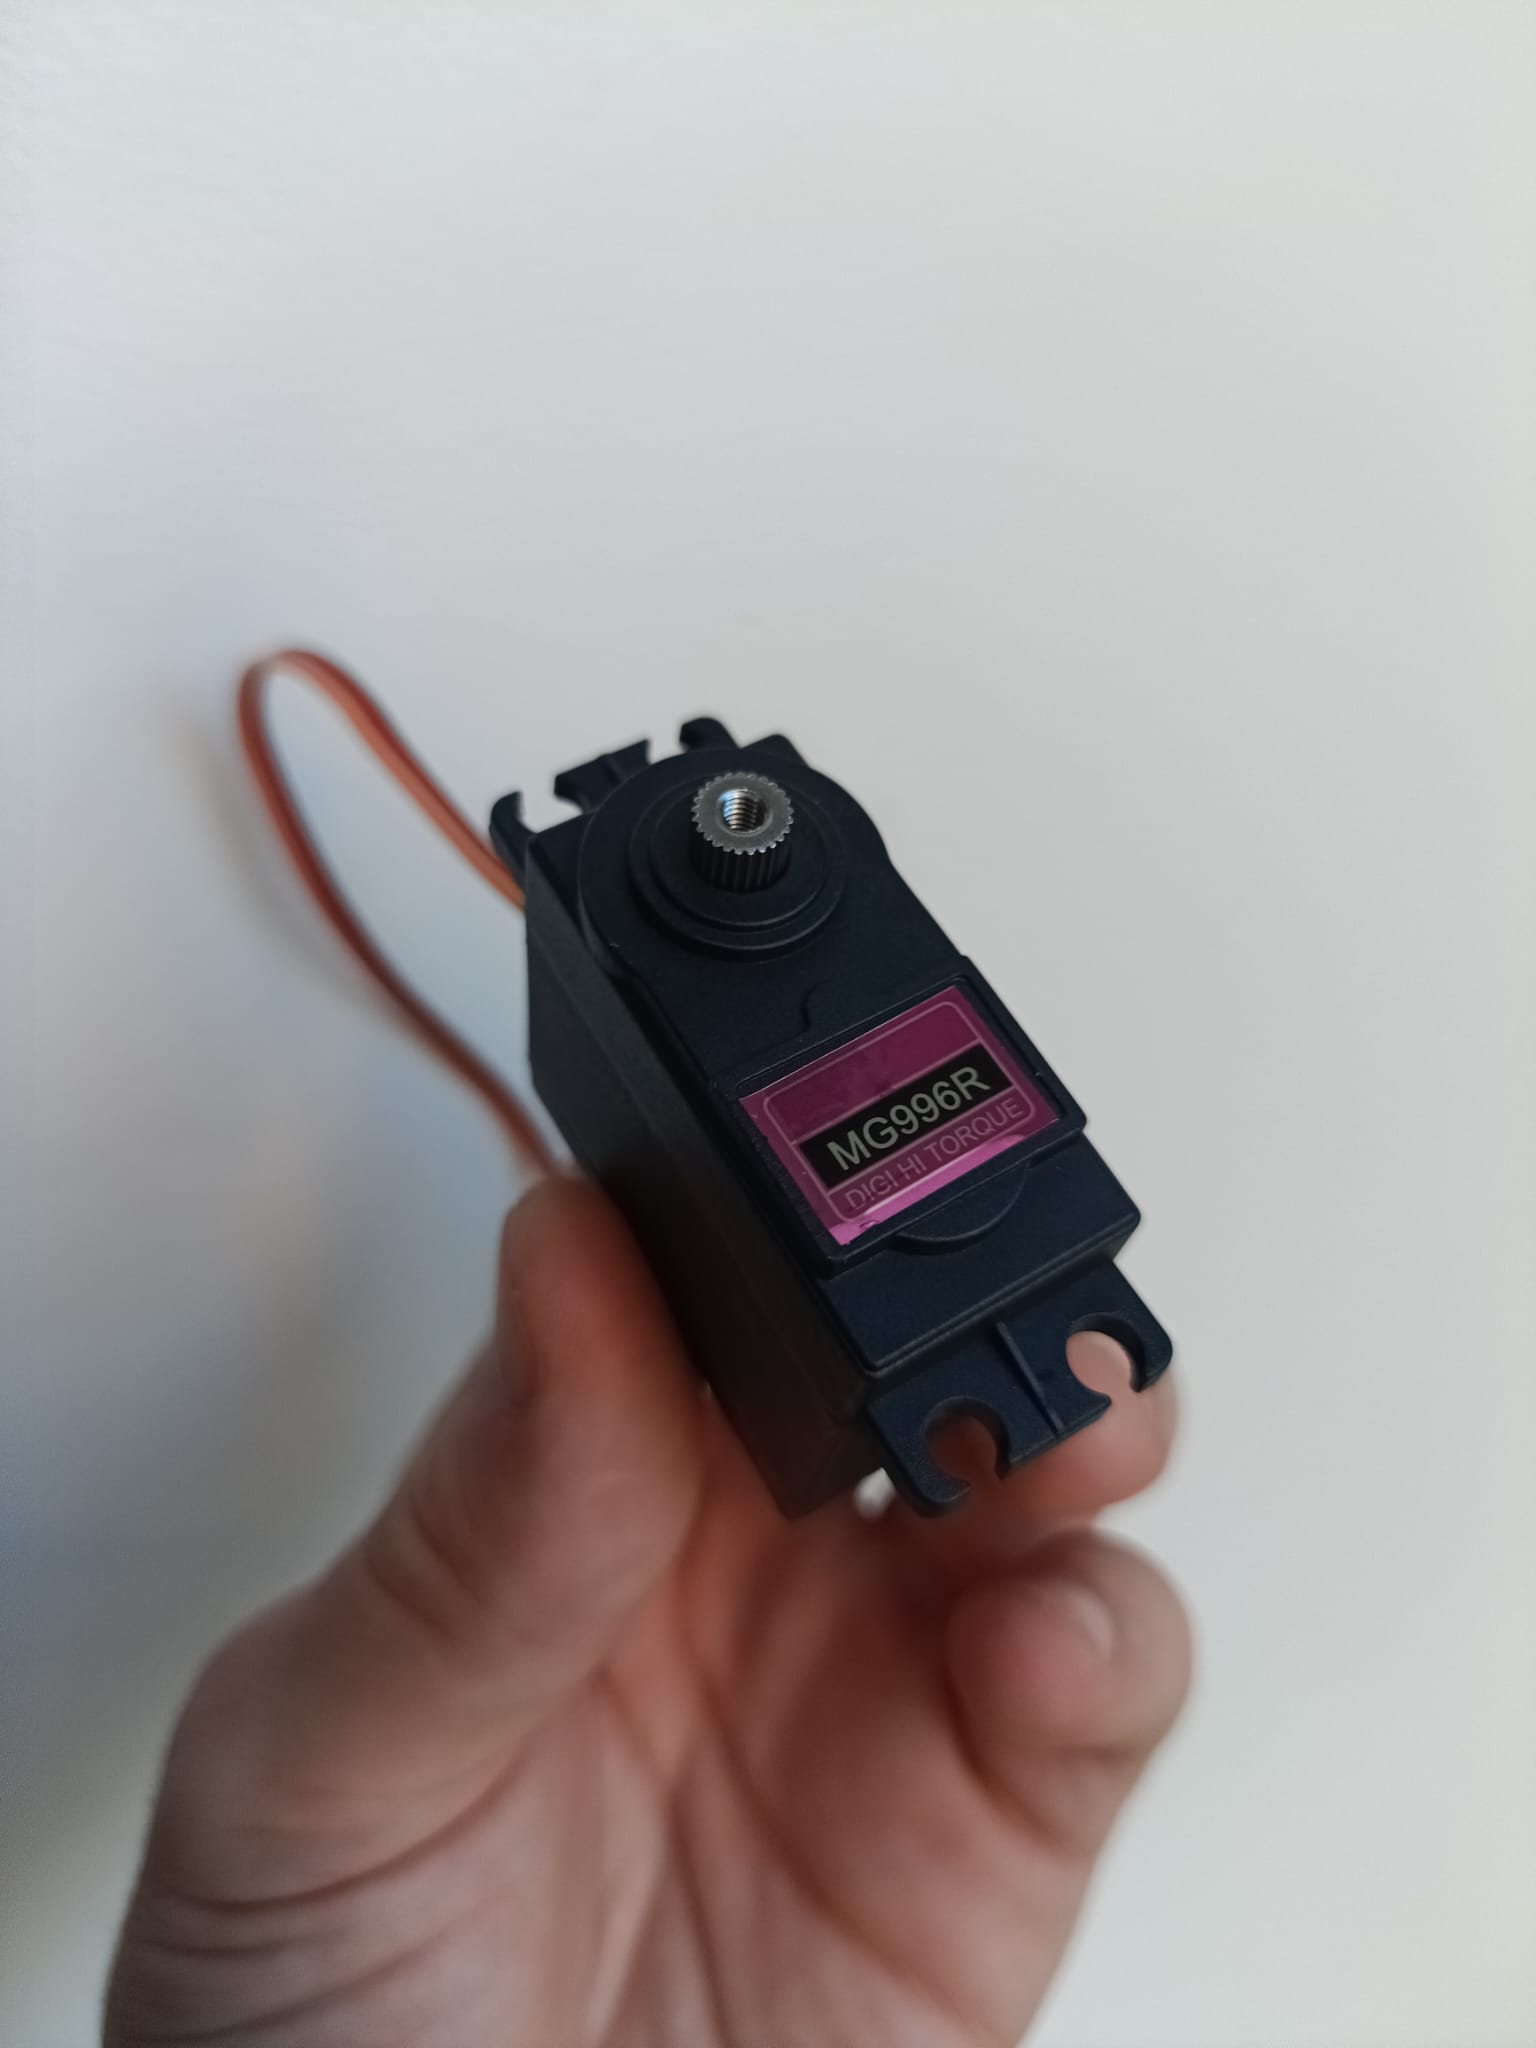
\includegraphics[width=0.5\textwidth]{figs/servo_mg996r.jpg}
	\caption{Servomotorul MG996R folosit pentru acționarea articulațiilor, cu
	angrenaje metalice și un cuplu de aproximativ 11~kg$\cdot$cm.}
	\label{fig:servo}
\end{figure}

Semnalul PWM care comandă un astfel de servomotor are o structură bine definită.
El este periodic, cu o perioadă de 20 de milisecunde, iar informația de poziție nu
este transmisă prin amplitudine, ci prin durata impulsului activ din cadrul
fiecărei perioade. Un impuls cu durata de aproximativ 1 milisecundă corespunde
poziției de la o extremă a cursei, un impuls de 2 milisecunde corespunde celeilalte
extreme, iar valorile intermediare determină proporțional unghiul dorit. Această
corespondență este ilustrată în Figura~\ref{fig:timing-pwm}, unde sunt suprapuse
cele trei cazuri reprezentative pentru pozițiile de 0, 90 și 180 de grade.

\begin{figure}[H]
	\centering
	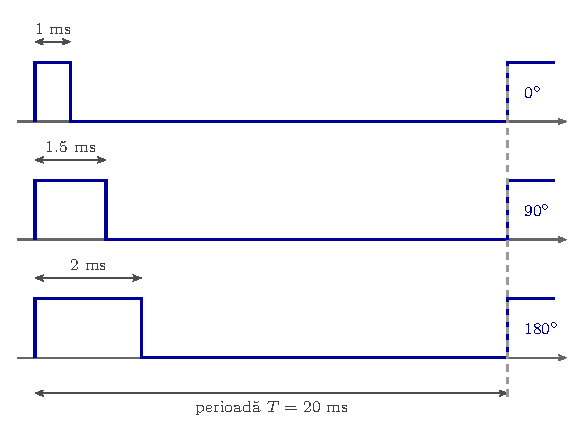
\includegraphics[width=0.8\textwidth]{figs/timing_pwm.pdf}
	\caption{Relația dintre durata impulsului și unghiul comandat. Un impuls de
	1~ms corespunde poziției de 0 grade, unul de 1,5~ms poziției de 90 de grade,
	iar unul de 2~ms poziției de 180 de grade, toate în cadrul aceleiași perioade
	de 20~ms.}
	\label{fig:timing-pwm}
\end{figure}

Relația dintre unghiul dorit $\alpha$, exprimat în grade, și durata impulsului
$\tau$, exprimată în milisecunde, este liniară și se scrie sub forma

\begin{equation}
\label{eq:pwm-pulse}
\tau(\alpha) = 1{,}0 + \frac{\alpha}{180} ,
\end{equation}

ceea ce înseamnă că la unghiul de 0 grade durata este de 1~ms, iar la 180 de grade
durata ajunge la 2~ms. Această durată trebuie tradusă într-un număr de perioade de
ceas, fiindcă generatorul PWM din interiorul plăcii numără impulsuri de ceas pentru
a măsura timpul. La frecvența de ceas a sistemului, de 100~MHz, o perioadă de ceas
durează 10 nanosecunde, astfel încât perioada completă de 20~ms corespunde la exact
două milioane de perioade de ceas, iar intervalul util al impulsului, de la 1 la
2~ms, se întinde pe o sută de mii de perioade de ceas.

Generatorul PWM funcționează pe baza unui numărător care parcurge ciclic valorile
corespunzătoare unei perioade de 20~ms. La fiecare ciclu, pentru fiecare canal, se
calculează un prag corespunzător unghiului dorit, iar ieșirea se menține la nivel
ridicat atâta timp cât numărătorul este sub acest prag și coboară la nivel scăzut
în rest. Astfel, durata impulsului activ este proporțională cu unghiul, exact cum
cere servomotorul. Rezoluția obținută în acest fel este mult mai fină decât
precizia mecanică a servomotorului, ceea ce înseamnă că pasul de cuantizare al
comenzii nu constituie un factor limitativ pentru precizia ansamblului. Faptul că
fiecare dintre cele opt canale dispune de propriul comparator, toate funcționând în
paralel, asigură generarea simultană a tuturor semnalelor, fără ca actualizarea
unui canal să o afecteze pe a celorlalte.

\section{Analiza temporală și sincronizarea}
\label{sec:analiza-timp}

Un sistem de control în timp real nu poate fi judecat doar după corectitudinea
algoritmilor, ci și după capacitatea de a-i executa în intervalul de timp
disponibil. Această secțiune analizează constrângerile temporale ale sistemului și
modul în care diferitele subsisteme, care lucrează la ritmuri foarte diferite, sunt
sincronizate între ele. Toate aceste aspecte pornesc de la ceasul de sistem al
plăcii, care funcționează la 100~MHz, ceea ce înseamnă o perioadă de ceas de exact
10 nanosecunde. Fiecare operație elementară din circuit se desfășoară pe parcursul
unuia sau mai multor astfel de intervale.

Referința temporală a întregului sistem este ciclul de control de 20~ms, impus de
servomotoare. La frecvența de 100~MHz, acest ciclu corespunde la exact două
milioane de perioade de ceas, fiindcă produsul dintre frecvență și durată dă
$100 \times 10^6 \times 0{,}02 = 2\,000\,000$. Acesta este, practic, bugetul de
timp în interiorul căruia trebuie să încapă toate operațiile dintr-un ciclu, de la
recepția datelor până la actualizarea semnalelor de ieșire. Cum se va vedea, acest
buget este extrem de generos în raport cu necesarul real de calcul.

\subsection{Sincronizarea datelor între subsisteme}

O dificultate aparte a sistemului provine din faptul că subsistemele sale lucrează
la ritmuri diferite și independente. Pe de o parte, cadrele cu unghiuri sosesc prin
UART la momente dictate de calculatorul gazdă și de procesul de detecție vizuală,
fără nicio legătură cu ciclul intern al plăcii. Pe de altă parte, filtrul Kalman și
generatorul PWM lucrează strict ritmate de ciclul de 20~ms. Dacă filtrul ar citi
direct datele în curs de recepție, ar exista riscul ca un cadru să fie folosit pe
jumătate actualizat, în momentul în care un nou set de valori tocmai îl
suprascrie pe cel vechi, ceea ce ar produce comenzi eronate.

Pentru a evita această situație, între modulul de recepție și filtru a fost
introdus un mecanism de tip cutie poștală, care funcționează pe principiul dublului
tampon. Cadrele primite prin UART sunt scrise într-un prim registru, pe măsură ce
sosesc, și sunt însoțite de un fanion care indică prezența unor date noi.
Filtrul Kalman nu citește însă niciodată din acest registru direct. La începutul
fiecărui ciclu de 20~ms, dacă există date noi disponibile, conținutul primului
registru este copiat dintr-o singură mișcare într-un al doilea registru, din care
filtrul își preia valorile pe parcursul ciclului. În acest fel, filtrul lucrează
întotdeauna pe un set de date stabil și coerent, în timp ce recepția poate continua
nestingherită în fundal. Acest mecanism decuplează complet ritmul comunicației de
ritmul prelucrării și constituie elementul-cheie al sincronizării din sistem.

\subsection{Constrângerea impusă de convertorul analog-digital}

Și bucla de monitorizare prin convertorul analog-digital impune constrângeri
temporale proprii. Convertorul folosit este de tip sigma-delta, un tip de convertor
care obține o rezoluție foarte mare în schimbul unei rate de conversie mai
moderate. În configurația aleasă, cu un filtru digital de tip sinc de ordinul al
treilea, rata de ieșire a convertorului este de 50 de eșantioane pe secundă, ceea
ce se potrivește exact cu ciclul de control de 20~ms. Cu alte cuvinte, convertorul
furnizează o nouă măsurătoare de poziție pentru fiecare ciclu al sistemului, nici
mai des, nici mai rar decât este nevoie.

Comunicația cu convertorul se realizează prin interfața SPI, a cărei frecvență de
ceas a fost stabilită la 5~MHz, obținută prin divizarea ceasului de sistem de
100~MHz. Această valoare se încadrează confortabil sub limita maximă admisă de
convertor și asigură un transfer rapid al celor câțiva octeți necesari pentru
citirea unei conversii. Un detaliu important al acestei interfețe este sincronizarea
semnalului de intrare provenit de la convertor. Deoarece acest semnal vine dintr-un
domeniu de timp diferit față de ceasul plăcii, el este trecut prin două bistabile
înseriate înainte de a fi folosit, o tehnică standard prin care se evită fenomenul
de metastabilitate, care ar putea altfel introduce valori eronate atunci când
semnalul se schimbă chiar în momentul citirii.

\subsection{Bugetul de calcul al filtrului Kalman}

Cea mai solicitantă operație din punct de vedere temporal este execuția filtrului
Kalman pentru toate cele opt canale. Filtrul este implementat ca o mașină cu stări,
care parcurge secvențial etapele de predicție și actualizare pentru fiecare canal,
efectuând o singură înmulțire pe ciclu de ceas pentru a respecta constrângerile de
timp. Operația cea mai costisitoare este împărțirea necesară la calculul câștigului
Kalman, realizată printr-un algoritm secvențial care produce câte un bit de rezultat
pe ciclu de ceas și necesită câteva zeci de cicluri pentru a se finaliza. Întrucât
pentru fiecare canal sunt necesare două astfel de împărțiri, prelucrarea unui singur
canal ocupă de ordinul a o sută cincizeci de cicluri de ceas, iar tratarea tuturor
celor opt canale necesită, în total, aproximativ o mie două sute de cicluri.

La o perioadă de ceas de 10 nanosecunde, acest necesar se traduce într-un timp de
calcul de ordinul a 12 până la 13 microsecunde pentru întregul set de canale.
Trebuie subliniat că această valoare este o estimare, nu o cifră fixă, deoarece
numărul exact de cicluri variază de la un ciclu la altul. Atunci când o măsurătoare
diferă foarte mult de predicție, filtrul ocolește o parte din calcule și reia
estimarea, iar algoritmul de împărțire poate să se încheie mai devreme în anumite
situații. Indiferent de aceste variații însă, timpul de calcul rămâne de ordinul
microsecundelor, cu mult sub bugetul de 20 de milisecunde disponibil pentru un
ciclu. Practic, filtrul ocupă o fracțiune neglijabilă din timpul unui ciclu, ceea
ce lasă o marjă uriașă pentru eventuale extinderi viitoare ale sistemului.

Din această analiză rezultă o observație importantă. Constrângerea reală a
sistemului nu este debitul de calcul, care este oricum acoperit cu prisosință, ci
închiderea temporală a circuitului la frecvența de 100~MHz. Cu alte cuvinte,
provocarea nu constă în a încadra calculele în cele 20~ms, lucru evident
îndeplinit, ci în a asigura că fiecare operație elementară se încheie în interiorul
unei singure perioade de ceas de 10 nanosecunde, astfel încât circuitul să poată
funcționa stabil la această frecvență. Operația de împărțire, în special, ridică
dificultăți în acest sens, fiindcă o realizare directă a ei ar avea o cale
combinațională prea lungă pentru a se încadra într-o perioadă de ceas. Modul în
care această problemă a fost rezolvată, prin descompunerea împărțirii pe mai multe
cicluri și prin alte tehnici de reducere a căilor combinaționale, este tratat în
detaliu în capitolul de proiectare și implementare.

\section{Fundamentarea alegerii componentelor}
\label{sec:analiza-componente}

Ultima parte a acestui capitol tratează raționamentul teoretic care a stat la baza
alegerii principalelor componente electronice ale sistemului. Spre deosebire de
descrierea concretă a montajului, care aparține capitolului de proiectare, aici sunt
discutate principiile care au impus utilizarea fiecărui tip de componentă. Un fir
roșu al acestor decizii îl reprezintă protejarea părții digitale a sistemului și
asigurarea unei alimentări curate, în condițiile în care motoarele introduc
perturbații importante.

\subsection{Necesitatea izolării galvanice}

Cea mai importantă decizie de proiectare la nivel electronic este separarea
domeniului digital de cel de putere prin izolare galvanică. Placa FPGA lucrează cu
semnale logice de mică putere și este sensibilă la perturbații, în timp ce
servomotoarele consumă curenți importanți și produc, prin natura motoarelor
electrice, vârfuri de tensiune și zgomot electric atunci când pornesc, se opresc
sau întâmpină rezistență. Dacă cele două domenii ar împărți aceeași masă electrică,
aceste perturbații s-ar propaga înapoi în placă și ar putea provoca funcționări
eronate sau chiar deteriorarea circuitului. Izolarea galvanică întrerupe complet
legătura electrică directă dintre cele două domenii, permițând totuși transmiterea
semnalelor, astfel încât informația trece dintr-o parte în alta fără ca
perturbațiile de putere să poată ajunge la partea sensibilă.

Pentru izolarea celor opt semnale PWM care comandă servomotoarele se folosesc
izolatoare digitale de tip ADuM1400~\cite{adum1400_eval}. Acestea
sunt izolatoare cu patru canale, bazate pe tehnologia iCoupler, în care semnalul
este transmis peste bariera de izolare prin intermediul unor transformatoare
miniaturale integrate în cip, nu prin cuplaj optic precum la optocuploarele
clasice. Structura internă a circuitului este ilustrată în
Figura~\ref{fig:adum-diagrama}, unde se observă cele patru canale, fiecare format
dintr-un bloc de codare, un transformator care realizează trecerea peste bariera
de izolare și un bloc de decodare. Această tehnologie oferă un consum redus și o
stabilitate bună în timp. Deoarece un singur circuit dispune de patru canale, iar
sistemul are nevoie de opt semnale PWM, se folosesc două astfel de circuite, care
împreună acoperă toate cele opt canale de comandă către servomotoare.

\begin{figure}[H]
	\centering
	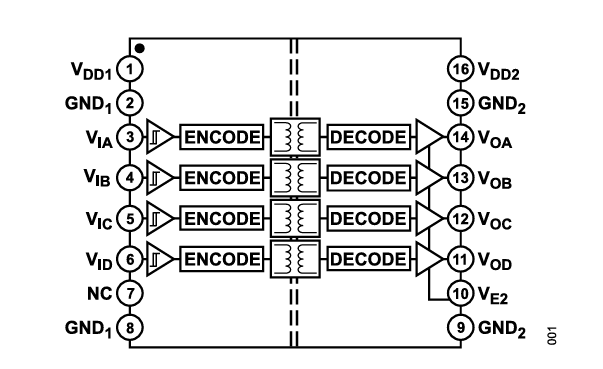
\includegraphics[width=0.7\textwidth]{figs/adi_adum_diagrama.png}
	\caption{Structura internă a izolatorului ADuM1400, cu cele patru canale.
	Fiecare canal transmite semnalul peste bariera de izolare printr-un
	transformator miniatural, conform tehnologiei iCoupler.}
	\label{fig:adum-diagrama}
\end{figure}

Pentru testarea și integrarea acestor izolatoare a fost folosită placa de
evaluare prezentată în Figura~\ref{fig:adum-eval}, pe care se montează circuitul
propriu-zis și care expune toate conexiunile necesare, ușurând astfel realizarea
montajului experimental.

\begin{figure}[H]
	\centering
	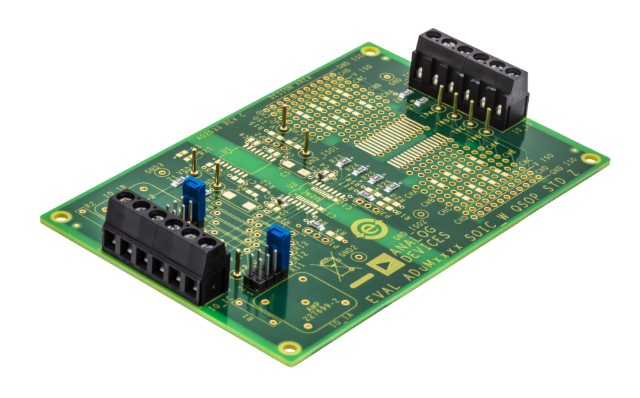
\includegraphics[width=0.6\textwidth]{figs/adi_adum_eval.jpg}
	\caption{Placa de evaluare pe care se montează izolatorul ADuM1400~\cite{adumqs_eval}, cu
	conexiunile aduse la borne accesibile pentru integrarea în montaj.}
	\label{fig:adum-eval}
\end{figure}

Bucla de monitorizare prin convertorul analog-digital trebuie la rândul ei izolată,
fiindcă altfel ar reintroduce o legătură directă între domeniul de putere și placă,
anulând efectul izolării de pe calea de comandă. Magistrala SPI prin care
comunică convertorul este izolată cu ajutorul circuitului MAX14850~\cite{max14850_eval}, prezentat în
Figura~\ref{fig:max}. Acesta este un izolator digital cu șase canale, dintre care
patru unidirecționale și două bidirecționale, ceea ce îl face deosebit de potrivit
pentru izolarea unei magistrale SPI, care necesită mai multe linii de semnal în
ambele sensuri. Astfel, întregul lanț de feedback rămâne separat galvanic de partea
de putere, păstrând integritatea izolării întregului sistem.

\begin{figure}[H]
	\centering
	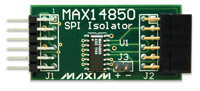
\includegraphics[width=0.45\textwidth]{figs/adi_max14850.png}
	\caption{Izolatorul digital cu șase canale MAX14850, folosit pentru izolarea
	magistralei SPI dintre convertorul analog-digital și placa FPGA.}
	\label{fig:max}
\end{figure}

\subsection{Convertorul analog-digital de precizie}

Citirea poziției reale a servomotoarelor necesită un convertor analog-digital
capabil să măsoare cu precizie tensiuni mici, eventual afectate de zgomot. Pentru
acest rol a fost ales convertorul AD7124-8~\cite{ad7124_eval}, prezentat în Figura~\ref{fig:ad7124}.
Este un convertor de tip sigma-delta cu o rezoluție de 24 de biți, ceea ce îi
conferă o gamă dinamică foarte mare și o sensibilitate ridicată. Spre deosebire de
convertoarele rapide, cu aproximații succesive, un convertor sigma-delta obține
această precizie ridicată prin supraeșantionare și filtrare digitală, fiind ideal
pentru semnale care variază lent, așa cum este poziția unui servomotor. Convertorul
dispune de mai multe canale de intrare, ceea ce permite citirea mai multor
servomotoare cu un singur circuit, și de un filtru digital configurabil, prin care
rata de conversie a fost potrivită exact cu ciclul de control al sistemului.

\begin{figure}[H]
	\centering
	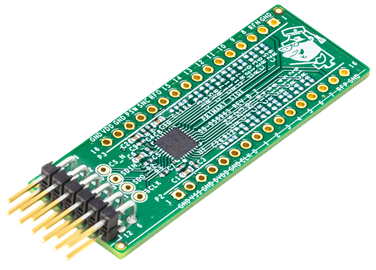
\includegraphics[width=0.5\textwidth]{figs/adi_ad7124.png}
	\caption{Convertorul analog-digital sigma-delta pe 24 de biți AD7124-8, folosit
	pentru citirea poziției reale a servomotoarelor.}
	\label{fig:ad7124}
\end{figure}

\subsection{Alimentarea sistemului}

Funcționarea corectă a întregului ansamblu depinde și de o alimentare bine
dimensionată, capabilă să furnizeze atât curentul mare cerut de servomotoare, cât
și o tensiune curată pentru partea sensibilă de măsurare. Cele opt servomotoare,
mai ales atunci când acționează simultan sub sarcină, solicită un curent
considerabil, motiv pentru care alimentarea lor se face printr-un regulator capabil
de un curent ridicat, realizat cu modulul DC2468A~\cite{dc2468a_eval}, prezentat în
Figura~\ref{fig:dc2468a}. Acesta coboară tensiunea sursei la valoarea de 5~V cerută
de servomotoare, furnizând un curent suficient pentru ca toate motoarele să poată
funcționa simultan fără căderi de tensiune.

\begin{figure}[H]
	\centering
	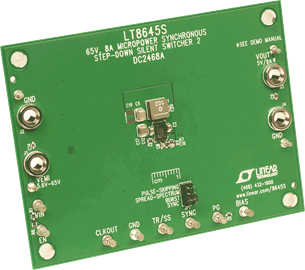
\includegraphics[width=0.5\textwidth]{figs/adi_dc2468a.png}
	\caption{Modulul de alimentare DC2468A, care furnizează tensiunea de 5~V și
	curentul ridicat necesar celor opt servomotoare.}
	\label{fig:dc2468a}
\end{figure}

Convertorul analog-digital, fiind un circuit de precizie, necesită o alimentare cât
mai curată, lipsită de zgomot. Pentru aceasta se folosește un regulator liniar de
tip ADP165~\cite{adp165_eval}, prezentat în Figura~\ref{fig:adp165}, care coboară tensiunea de 5~V la
cea de 3,3~V folosită de convertor. Spre deosebire de regulatoarele în comutație,
care sunt eficiente dar introduc zgomot, un regulator liniar furnizează o tensiune
foarte stabilă și curată, esențială pentru a nu compromite precizia măsurătorilor
convertorului. În felul acesta, fiecare parte a sistemului primește exact tipul de
alimentare de care are nevoie, partea de putere fiind alimentată eficient, iar cea
de măsurare fiind alimentată curat.

\begin{figure}[H]
	\centering
	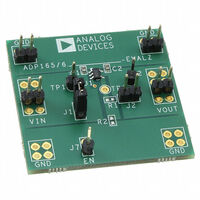
\includegraphics[width=0.45\textwidth]{figs/adi_adp165.png}
	\caption{Regulatorul liniar ADP165, care furnizează tensiunea curată de 3,3~V
	necesară convertorului analog-digital.}
	\label{fig:adp165}
\end{figure}

\vspace{0.5cm}
\noindent
Fundamentele teoretice prezentate în acest capitol, de la structura logică a
sistemului și principiul de acționare a mâinii, până la modelul filtrului Kalman,
aritmetica folosită, controlul servomotoarelor, analiza temporală și raționamentul
alegerii componentelor, constituie baza pe care se sprijină proiectarea de detaliu.
Capitolul următor reia aceste elemente din perspectiva implementării concrete,
arătând cum au fost transpuse în structura hardware a plăcii și în ansamblul fizic
al mâinii robotice.
